\documentclass[slidestop,compress,14pt,xcolor=dvipsnames]{beamer}\usepackage[]{graphicx}\usepackage[]{color}
%% maxwidth is the original width if it is less than linewidth
%% otherwise use linewidth (to make sure the graphics do not exceed the margin)
\makeatletter
\def\maxwidth{ %
  \ifdim\Gin@nat@width>\linewidth
    \linewidth
  \else
    \Gin@nat@width
  \fi
}
\makeatother

\definecolor{fgcolor}{rgb}{0.345, 0.345, 0.345}
\newcommand{\hlnum}[1]{\textcolor[rgb]{0.686,0.059,0.569}{#1}}%
\newcommand{\hlstr}[1]{\textcolor[rgb]{0.192,0.494,0.8}{#1}}%
\newcommand{\hlcom}[1]{\textcolor[rgb]{0.678,0.584,0.686}{\textit{#1}}}%
\newcommand{\hlopt}[1]{\textcolor[rgb]{0,0,0}{#1}}%
\newcommand{\hlstd}[1]{\textcolor[rgb]{0.345,0.345,0.345}{#1}}%
\newcommand{\hlkwa}[1]{\textcolor[rgb]{0.161,0.373,0.58}{\textbf{#1}}}%
\newcommand{\hlkwb}[1]{\textcolor[rgb]{0.69,0.353,0.396}{#1}}%
\newcommand{\hlkwc}[1]{\textcolor[rgb]{0.333,0.667,0.333}{#1}}%
\newcommand{\hlkwd}[1]{\textcolor[rgb]{0.737,0.353,0.396}{\textbf{#1}}}%

\usepackage{framed}
\makeatletter
\newenvironment{kframe}{%
 \def\at@end@of@kframe{}%
 \ifinner\ifhmode%
  \def\at@end@of@kframe{\end{minipage}}%
  \begin{minipage}{\columnwidth}%
 \fi\fi%
 \def\FrameCommand##1{\hskip\@totalleftmargin \hskip-\fboxsep
 \colorbox{shadecolor}{##1}\hskip-\fboxsep
     % There is no \\@totalrightmargin, so:
     \hskip-\linewidth \hskip-\@totalleftmargin \hskip\columnwidth}%
 \MakeFramed {\advance\hsize-\width
   \@totalleftmargin\z@ \linewidth\hsize
   \@setminipage}}%
 {\par\unskip\endMakeFramed%
 \at@end@of@kframe}
\makeatother

\definecolor{shadecolor}{rgb}{.97, .97, .97}
\definecolor{messagecolor}{rgb}{0, 0, 0}
\definecolor{warningcolor}{rgb}{1, 0, 1}
\definecolor{errorcolor}{rgb}{1, 0, 0}
\newenvironment{knitrout}{}{} % an empty environment to be redefined in TeX

\usepackage{alltt}
\usepackage{lmodern}
\usepackage{graphicx} %package for attaching images
%\usetheme{Madrid}
\usetheme{Ilmenau}
 %verbatim
\mode<presentation>
\setbeamercolor{section in head}{parent=palette quaternary}

\makeatletter
\setbeamertemplate{}
{%
\vskip-9ex%
\begin{beamercolorbox}{}
\hfill\usebeamercolor[fg]{navigation symbols dimmed}%
    \insertslidenavigationsymbol
    \insertframenavigationsymbol
    \insertsubsectionnavigationsymbol
    \insertsectionnavigationsymbol
    \insertdocnavigationsymbol
    \insertbackfindforwardnavigationsymbol
  \end{beamercolorbox}%    
  \begin{beamercolorbox}[ht=2ex,dp=3ex]{section in head}%
    \insertnavigation{\paperwidth}
  \end{beamercolorbox}%
}%
\makeatother

\author{Ken Mwai}
\institute{Pwani-University R WorkShop}
\IfFileExists{upquote.sty}{\usepackage{upquote}}{}

\begin{document}
\section{Correlation}
\begin{frame}{Title}
\vspace*{\fill}
\begin{center}
Correlation
\end{center}
\vspace*{\fill}
\end{frame}

\section{Overview}
\subsection{Introduction}
\begin{frame}{Overview}
\begin{itemize}
    \item  Correlation is made of {\bf Co- } (meaning "together"), and {\bf Relation }
    \item Statistical procedure used to measure and describe the relationship between two variables 
    \item Range between +1 and -1
      \begin{itemize}
        \item Positive when the values increase together
        \item Negative when one value decreases as the other increases 
      \end{itemize}
\ldots
\end{itemize}
\end{frame}
\begin{frame}{Overview cont..}
\begin{itemize}
  \item +1 is a perfect positive correlation
  \item 0 is no correlation (independence)
  \item -1 is a perfect negative correlation
\end{itemize}
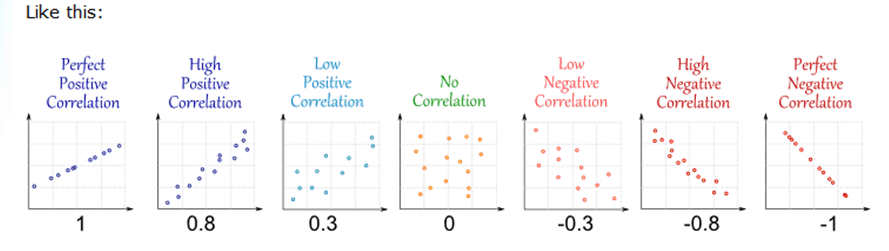
\includegraphics[scale=0.5]{corelation}
\end{frame}
\subsection{Uses}
\begin{frame}{Use of Corelation}
When two variables, let's call them X  Y, are correlated, then one variable can be
used to predict the other variable \newline
Example:IQ and perfomance...

\end{frame}

\section{Types}
\begin{frame}{Types}
\begin{itemize}
  \item {\bf Pearson product-moment correlation} -When both variables, X and Y, are continuous
  \item {\bf Point bi-serial correlation} - When 1 variable is continuous and 1 is dichotomous
  \item {\bf Phi coefficient} - When both variables are dichotomous
  \item {\bf Spearman rank correlation} - When both variables are ordinal (ranked data)
\end{itemize}
\end{frame}


\section{Calculation}
\begin{frame}{Calculation of Correlation}
defined as \newline 
\begin{center}
$r = S_{xy}/\sqrt{S_{xx}S_{yy}}.$ 
\end{center}
where 
\begin{center} $S_{xx} = \sum\limits_{i = 1}^N {\left( {x_i - \bar x} \right)^2}$ {(variance of x)} \end{center}
and
\begin{center} 
$S_{xy} = \sum\limits_{i = 1}^N {\left( {x_i - \bar x} \right)} {\left( {y_i - \bar y} \right)}$ {(covariance of x and y)}
\end{center}
\end{frame}


\section{Exercise}
\subsection{manual}
%\begin{frame}{Exercise - Desk Work}

%\begin{tabular}
\begingroup
\fontsize{7pt}{9pt}\selectfont



\begin{knitrout}
\definecolor{shadecolor}{rgb}{0.969, 0.969, 0.969}\color{fgcolor}\begin{kframe}
\begin{alltt}
\hlkwd{print}\hlstd{(df)}
\end{alltt}
\begin{verbatim}
##    temp icecream
## 1  14.2      215
## 2  16.4      325
## 3  11.9      185
## 4  15.2      332
## 5  18.5      406
## 6  22.1      522
## 7  19.4      412
## 8  25.1      614
## 9  23.4      544
## 10 18.1      421
## 11 22.6      445
## 12 17.2      408
\end{verbatim}
\end{kframe}
\end{knitrout}






%\end{tabular}
%\end{frame}

\subsection{Output}
%\begin{frame}{Another title}

\clearpage 

\begin{knitrout}
\definecolor{shadecolor}{rgb}{0.969, 0.969, 0.969}\color{fgcolor}\begin{kframe}
\begin{alltt}
\hlkwd{print}\hlstd{(df)}
\end{alltt}
\begin{verbatim}
##    temp icecream deviationTemp deviationIce      SSxy     SSxx     SSyy
## 1  14.2      215        -4.475     -187.417  838.6896 20.02563 35125.01
## 2  16.4      325        -2.275      -77.417  176.1229  5.17563  5993.34
## 3  11.9      185        -6.775     -217.417 1472.9979 45.90063 47270.01
## 4  15.2      332        -3.475      -70.417  244.6979 12.07563  4958.51
## 5  18.5      406        -0.175        3.583   -0.6271  0.03063    12.84
## 6  22.1      522         3.425      119.583  409.5729 11.73063 14300.17
## 7  19.4      412         0.725        9.583    6.9479  0.52562    91.84
## 8  25.1      614         6.425      211.583 1359.4229 41.28063 44767.51
## 9  23.4      544         4.725      141.583  668.9812 22.32562 20045.84
## 10 18.1      421        -0.575       18.583  -10.6854  0.33062   345.34
## 11 22.6      445         3.925       42.583  167.1396 15.40563  1813.34
## 12 17.2      408        -1.475        5.583   -8.2354  2.17563    31.17
\end{verbatim}
\begin{alltt}
\hlkwd{print}\hlstd{(sum.SSxy)}
\end{alltt}
\begin{verbatim}
## [1] 5325
\end{verbatim}
\begin{alltt}
\hlkwd{print}\hlstd{(sum.SSxx)}
\end{alltt}
\begin{verbatim}
## [1] 177
\end{verbatim}
\begin{alltt}
\hlkwd{print}\hlstd{(sum.SSyy)}
\end{alltt}
\begin{verbatim}
## [1] 174755
\end{verbatim}
\end{kframe}
\end{knitrout}




%\end{frame}
\section{Corelation}
\subsection{Corelation in R}
\clearpage
%\begin{frame}{Corelation in R}
\begin{knitrout}
\definecolor{shadecolor}{rgb}{0.969, 0.969, 0.969}\color{fgcolor}\begin{kframe}
\begin{alltt}
\hlkwd{cor}\hlstd{(df}\hlopt{$}\hlstd{temp, df}\hlopt{$}\hlstd{icecream)}
\end{alltt}
\begin{verbatim}
## [1] 0.9575
\end{verbatim}
\begin{alltt}
\hlkwd{cor.test}\hlstd{(df}\hlopt{$}\hlstd{temp, df}\hlopt{$}\hlstd{icecream)}
\end{alltt}
\begin{verbatim}
## 
## 	Pearson's product-moment correlation
## 
## data:  df$temp and df$icecream
## t = 10.5, df = 10, p-value = 1.016e-06
## alternative hypothesis: true correlation is not equal to 0
## 95 percent confidence interval:
##  0.8515 0.9883
## sample estimates:
##    cor 
## 0.9575
\end{verbatim}
\end{kframe}
\end{knitrout}

%\end{frame}
{\bf Diff btwn cor and cor.test}
The cor.test output also includes the point estimate reported by cor
Cor.test has p-value and also CI

\clearpage

\fontsize{12pt}{14pt}\selectfont

\subsection{Caution}
\begin{frame}{Caution}
\begin{itemize}
\item {\bf !"Correlation Is Not Causation" ... }\newline
When there is a correlation it does not mean that one thing causes the other
\item The magnitude of a correlation depends upon
many factors, including 
\begin{itemize}
\item Sampling (random and representative?)
\item Measurement of X and Y and Several other assumptions 
\ldots
\end{itemize}
\ldots
\end{itemize}
\end{frame}

\section{Assumptions}
\subsection{Assumptions}
\begin{frame}{Assumptions}
\begin{itemize}
    \item Normal Distribution for X and Y if not specifying the method - Use method="Spearman" for non-normal data.
    \item Linear relationship between X and Y
    \item {\bf Homoscedasticity} - homogeneity of variance/ uniformity of variance 
    leveneTest() from car package is used to test this
\end{itemize}
\end{frame}

\end{document}
